\documentclass{article}
\usepackage[margin=1in]{geometry}
\usepackage{amsmath,amsthm,amssymb}
\usepackage{bbm,enumerate,mathtools}
\usepackage{tikz,pgfplots}
\usepackage{chessboard}
\usepackage[hidelinks]{hyperref}
\usepackage{multicol} % Problem 35

\newenvironment{question}{\begin{trivlist}\item[\textbf{Question.}]}{\end{trivlist}}
\newenvironment{note}{\begin{trivlist}\item[\textbf{Note.}]}{\end{trivlist}}
\newenvironment{references}{\begin{trivlist}\item[\textbf{References.}]}{\end{trivlist}}
\newenvironment{related}{\begin{trivlist}\item[\textbf{Related.}]\end{trivlist}\begin{enumerate}}{\end{enumerate}}


\begin{document}
\rating{2}{1}
  Consider ways of nesting centered squares in the $n \times n$ square lattice.
\begin{figure}[ht!]
  \centering
  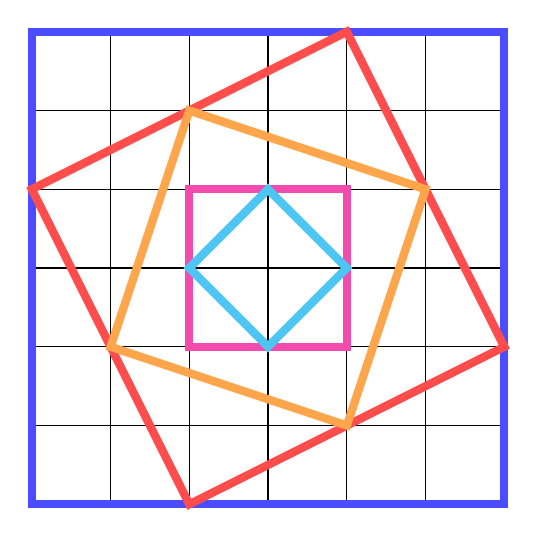
\begin{tikzpicture}
    \draw (0,0) grid (6,6);
    \draw[line width=3, blue!70] (0,0) rectangle (6,6);
    \draw[line width=3, red!70]  (0,4)--(4,6)--(6,2)--(2,0)--cycle;
    \draw[line width=3, orange!70]  (1,2)--(2,5)--(5,4)--(4,1)--cycle;
    \draw[line width=3, magenta!70]  (2,2) rectangle (4,4);
    \draw[line width=3, cyan!70]  (2,3)--(3,4)--(4,3)--(3,2)--cycle;
  \end{tikzpicture}
  ~~~
  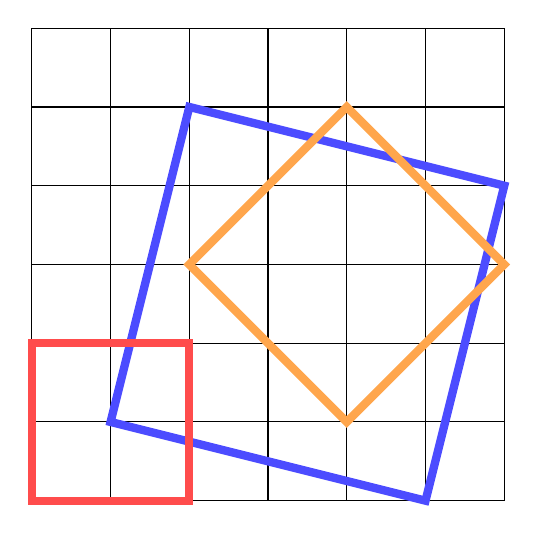
\begin{tikzpicture}
    \draw (1,1) grid (7,7);

      \draw[line width=3, blue!70] (6,1)--(7,5)--(3,6)--(2,2)--cycle;
      \draw[line width=3, red!70] (1,1)--(3,1)--(3,3)--(1,3)--cycle;
      \draw[line width=3, orange!70] (3,4)--(5,6)--(7,4)--(5,2)--cycle;
  \end{tikzpicture}
  \caption{
    An example of five non-parallel centered squares in the size 6 square, and
    an example of three non-parallel non-centered squares that do not share any
    lattice points.
  }
\end{figure}

\begin{question}
  What is the largest number of squares that can be nested?
\end{question}

\begin{related}
  \item What is the maximum sum of the areas? Perimeters?
  \item How many maximal configurations exist?
  \item What if the nested squares must be ``snug'', that is, all four of their
  corners must be on their outer neighbor.
  \item What if the nested squares cannot be parallel
    (i.e every square must be a scaling \textit{and} a rotation of another square)?
  \item What if they don't need to be centered, but instead no two squares can
    share a lattice point? If no two squares can be parallel?
  \item What if this is done on a triangular or hexagonal lattice?
\end{related}

\begin{references}
  \item Problems 21 and 66.
\end{references}

\end{document}
